\documentclass{article} % For LaTeX2e
\usepackage{nips15submit_e,times}
\usepackage{hyperref}
\usepackage{url}
\usepackage{graphicx}
\usepackage{amsfonts}
\usepackage{amssymb}
\usepackage{float}
\usepackage{listings}
\usepackage{xcolor}
\usepackage{amsmath}
%\documentstyle[nips14submit_09,times,art10]{article} % For LaTeX 2.09


\title{Problem Set 4 for Machine Learning 15 Fall}


\author{
Jingyuan Liu\\
AndrewId: jingyual\\
\texttt{jingyual@andrew.cmu.edu} \\
}


\newcommand{\fix}{\marginpar{FIX}}
\newcommand{\new}{\marginpar{NEW}}
\newcommand{\argmin}{\arg\!\min}
\newcommand{\norm}[1]{\left\lVert #1 \right\rVert}
\newcommand{\abs}[1]{\left\lvert #1 \right\rvert}
\newcommand{\inner}[1]{\left\langle #1 \right\rangle}


\nipsfinalcopy % Uncomment for camera-ready version


\begin{document}
\maketitle



\section{VC dimension}


\subsection{Show the VC dimension of linear classifier}
To prove that the linear classifier h with x in $ R^n $ has the VC dimension of
n + 1, we need to prove that $VCdim(h_n) >= n + 1$, and then prove that
$VCdim(h_n) <= n + 1$.

\textbf{(a). Prove $VCdim(h_n) >= n+1$}

First of all, we could use the Mathematical Induction to prove that $VCdim(H) >=
n+1$:

For n = 1, it is easy to get $VCdim(h_1) >= 2$

For n = 2, we could also get $VCdim(h_2) >= 3$, which could be proved using following figures:

\begin{figure}[!htbp]
\begin{center}
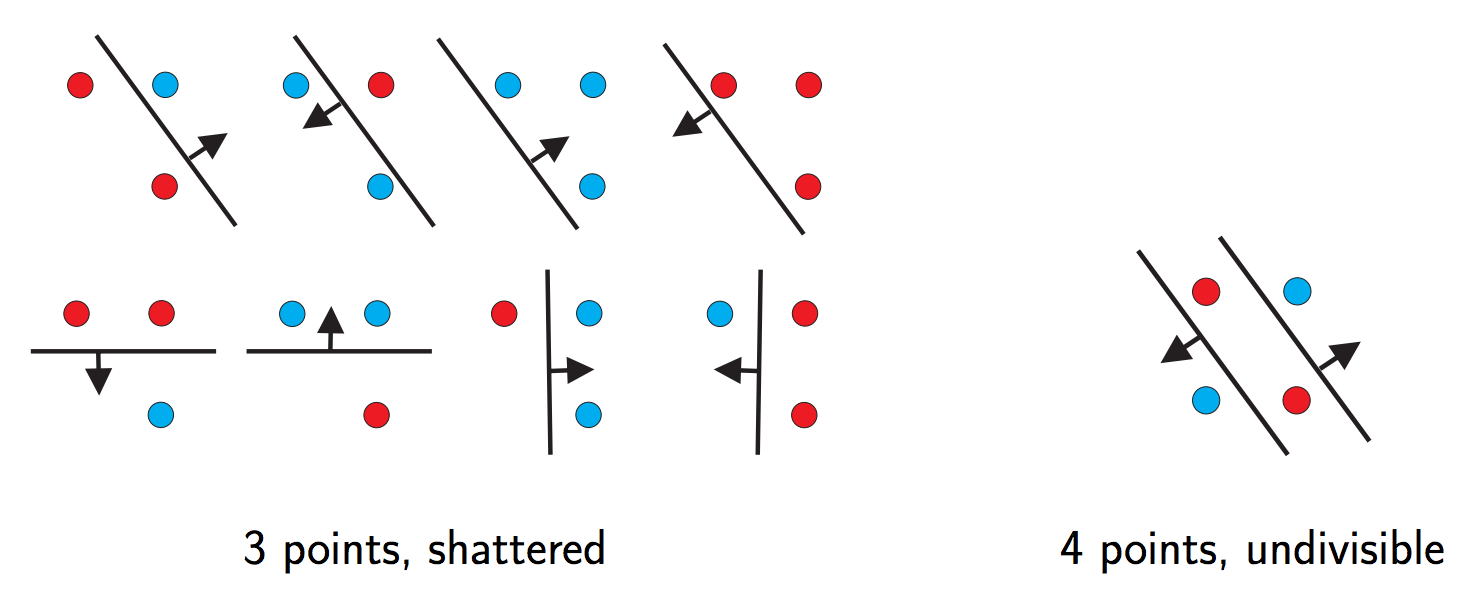
\includegraphics[width=60mm]{pic/q11.png}
\end{center}
\caption{The representation of $VCdim(h_2)$}
\end{figure}

For n = i, we assume that the $VCdim(h_i) >= i+1$. We could form a matrix of
(i+1)*(i+1),
with the rank of i+1, since the VCdim is i+1.

For n = i+1, we could form a matrix of (i+2)*(i+2), since the variable
x have one more independent dimension. Therefore, $VCdim(h_{i+1}) >= VCdim(h_i) + 1
>= i+2$.

Therefore, we have $VCdim(h_n) >= n+1$.

\textbf{(b). Prove $VCdim(h_n) <= n+1$}

Then we should prove that $VCdim(h_n) <= n+1$:

Suppose we could shatter n+2 points, then using the convex combinations of
points in C, we could seperate points into S1 and S2, that:

\begin{equation}
conv(s1) \cap conv(s2) \neq \emptyset
\end{equation}

However, if $VCdim(h_n) = n+2$, then we could spilt points to half space
contains s1 and the complement of the half space contains s2. This implies that
the both half space contains the convex hull of s1 and the complement of the
half space the contains the convex hull of s2. Thus, we get:

\begin{equation}
conv(s1) \cap conv(s2) = \emptyset
\end{equation}

These two observations are contradictory to each other. So we know that for the
n+2 points here, we could not use the linear classifier to shatter all of them.

\textbf{In conclusion}, we prove that $VCdim(h_n) >= n+1$ and $VCdim(h_n) <= n+1$ for the
linear classifier, then we have $VCdim(h_n) = n+1$


\subsection{Show the VC dimension of axis-aligned boxes}

Similarily, for this case, to prove that the axis-aligned boxes classifier h
with x in $ R^n $ has the VC dimension of 2n, we need to prove that
$VCdim(h_n) >= 2n$, and then prove that $VCdim(h_n) <= 2n$.

\textbf{(a). Prove $VCdim(h_n) >= 2n$}

First of all, we need to prove that for any case, $VCdim(h_n) >= 2n$, which
means if the x has n dimensions, we can use the axis-aligned boxes classifiers
to shatter 2n points.

Suppose we have n dimensions, then we can map all the x to a dimension i. In the
dimension i, we can have $x^i_{max}$ and $x^i_{min}$. Therefore, in this
dimension i, we could always shatter at least 2 points via a split between the
$x^i_{max}$ and $x^i_{min}$.

Considering we have n dimensions, and the mapping of each dimension of the data is
independent to the mapping of other dimension of the data. Therefore, we could
at least shatter 2*n points via the axias-alighed boxes. Therefore, we have
$VCdim(h_n) >= 2n$.

\textbf{(b). Prove $VCdim(h_n) <= 2n$}

Then we need to prove that $VCdim(h_n) <= 2n$. Suppose we have 2n + 1 points, we
could always find the 2n ``boundries'', which is the min value and max value for
each dimension, and form an ``area''. Then the 2n+1th points will be guaranteed to
appear within the selected ``area''.

For any 2n+1 points, we could always transfer to the above mentioned scenario. In
this scenario, we could not classify the 2n+1th point, because it is contained
within the ``area'', and no rules are guaranteed to rightly classify it.

Therefore, by mapping the data to each dimension and form an ``area'', we could
prove that $VCdim(h_n) <= 2n$.

\textbf{In conclusion}, we prove that $VCdim(h_n) >= 2n$ and $VCdim(h_n) <= 2n$ for the
axis-alighed boxes, then we have $VCdim(h_n) = 2n$



\section{Support Vector Machines}


\subsection{Support Vector Regression}

\textbf{2.1.1. write the dual problem}

Suppose we have $\xi_i$ ofr each $x_i$:

\begin{equation}
\abs{f(x) - y} < \epsilon
\end{equation}

\begin{equation}
- \epsilon  < w^T x_i - y_i < \epsilon
\end{equation}

Let's set:

\begin{equation}
\abs{w^T x_i - y_i} - \epsilon = \xi_i
\end{equation}

\begin{equation}
L = \frac{1}{2} \norm{w}_2^2 + C \sum_{i=1} \xi_i 
- \sum_i \alpha_i (\epsilon + \xi_i - y_i + w x_i)
- \sum_i \alpha_i^{\star} (\epsilon + \xi_i +y_i - w x_i)
- \sum_i \beta_i \xi_i
\end{equation}

\begin{equation}
\alpha_i >= 0, \alpha_i^{\star} >= 0, \beta_i >= 0
\end{equation}

We have to satisfy saddle constraints condition, so

\begin{equation}
\partial_w L = w - \sum_i (\alpha_i - \alpha_i^{\star}) x_i = 0
\end{equation}

\begin{equation}
\partial_{\xi_i} L = C - \alpha_i -\alpha_i^{\star} - \beta_i = 0
\end{equation}

Take the the conditions back and we can get the form of dual problem of SVR:

\begin{equation}
maximize: - \frac{1}{2} \sum_{i,j=1} (\alpha_i - \alpha_i^{\star})
(\alpha_j - \alpha_j^{\star}) x_i^T x_j
- \epsilon \sum_i (\alpha_i + \alpha_i^{\star})
+ \sum_i y_i (\alpha_i - \alpha_i^{\star})
\end{equation}

\begin{equation}
subject \quad to: \sum_i (\alpha_i - \alpha_i^{\star}) = 0, \qquad
\alpha_i, \alpha_i^{\star} \in [ 0, C]
\end{equation}


\textbf{2.1.2. KKT Conditions}

The KKT condition for this problem is:

\begin{equation}
\partial_w L = w - \sum_i (\alpha_i - \alpha_i^{\star}) x_i = 0
\end{equation}

\begin{equation}
\partial_{\xi_i} L = C - \alpha_i -\alpha_i^{\star} - \beta_i = 0
\end{equation}

\begin{equation}
\epsilon + \xi_i - y_i + w^T x_i >= 0
\end{equation}

\begin{equation}
\epsilon + \xi_i^{\star} + y_i - w^T x_i >= 0
\end{equation}

\begin{equation}
\alpha_i >= 0, \alpha_i^{\star} >= 0, \beta_i >=0
\end{equation}

\begin{equation}
\alpha_i (\epsilon + \xi_i - y_i + w^T x_i) = 0
\end{equation}

\begin{equation}
\alpha_i^{\star} (\epsilon + \xi_i^{\star} + y_i - w^T x_i) = 0
\end{equation}

\textbf{2.1.3. Kernelized SVR}

The prediction rule is:

\begin{equation}
w = \sum_i (\alpha_i - \alpha_i^{\star}) x_i
\end{equation}

\begin{equation}
f(x) = \sum_i (\alpha_i - \alpha_i^{\star}) x_i^T x
\end{equation}

Add we can use kernel to transfer the x, therefore:

\begin{equation}
f(x_j) = \sum_i (\alpha_i - \alpha_i^{\star}) K(x_i, x_j)
\end{equation}

\textbf{2.1.4. Why using SVR primal}


We are using the primal of SVM and the dual of SVR, this is because we want to
compose the term:

\begin{equation}
\sum_i x_i x
\end{equation}

Therefore, we could use the kernel trick to implicitly transfer the feature of
the data to other spaces.


\subsection{Support Kernel Machines}

\textbf{2.2.1.(a) The minimum of the Lagrangian function}

Given L, the Lagrangian function, we could derive to optimize the w:

\begin{equation}
\frac{\partial L}{\partial w_j} = \frac{1}{2} \frac{\partial (\sum_j d_j
\norm{w_i}_2)^2}{\partial w_j} - \frac{\partial \alpha_i y_i \sum_j w_j^T
x_{ji}}{\partial w_j}
\end{equation}

We can have $\frac{\partial L}{\partial w_j} = 0$. Then we can both times the
$w_j^T$:

\begin{equation}
\frac{w_j d_j \sum_j \norm{w_j}_2 d_j }{\norm{w_j}_2} = \sum_i \alpha_i y_i x_{ji}
\end{equation}

\begin{equation}
\norm{w_j}_2 d_j \gamma = w_j^T \sum_i \alpha_i y_i x_{ji}
\end{equation}

\textbf{2.2.1.(b) Show that $\norm{\sum_i \alpha_i y_i x_{ji}}_2 < d_j \gamma$}

In the last section, we have:

\begin{equation}
\frac{w_j d_j \sum_j \norm{w_j}_2 d_j }{\norm{w_j}_2} = \sum_i \alpha_i y_i x_{ji}
\end{equation}

Therefore, when the w is not 0, we can take the l2-norm of the this two vectors
and get:

\begin{equation}
\norm{\frac{w_j d_j \sum_j \norm{w_j}_2 d_j }{\norm{w_j}_2}}_2
= \norm{\sum_i \alpha_i y_i x_{ji}}_2
\end{equation}

Because w is a vector, we know that:

\begin{equation}
\norm{\frac{w_j}{\norm{w_j}_2}}_2 = 1
\end{equation}

So we have:

\begin{equation}
\norm{w_j}_2 d_j \gamma = w_j^T \sum_i \alpha_i y_i x_{ji}
\end{equation}

\textbf{2.2.1.(c) Show that}

For the first point, from the previous problem, we would know that:

\begin{equation}
\norm{\sum_i \alpha_i y_i x_{ji}}_2 <= d_j \gamma
\end{equation}

And we have also proven that, when w is not zero:

\begin{equation}
\norm{\sum_i \alpha_i y_i x_{ji}}_2 = d_j \gamma
\end{equation}

Then with the $w_j = 0$, we should have:

\begin{equation}
\norm{\sum_i \alpha_i y_i x_{ji}}_2 < d_j \gamma
\end{equation}

For the second point, we would know that:

\begin{equation}
\frac{w_j d_j \sum_j \norm{w_j}_2 d_j }{\norm{w_j}_2} = \sum_i \alpha_i y_i x_{ji}
\end{equation}

\begin{equation}
w_j = \frac{\norm{w_j}_2}{d_j \gamma} \sum_i \alpha_i y_i x_ji
\end{equation}

We could know that $\norm{w_j}_2 > 0, d_j>0, \gamma>0$, therefore, we could
always have a $\eta_i$:

\begin{equation}
w_j = \eta_j \sum_i \alpha_i y_i x_{ji}, \eta_j > 0
\end{equation}

When $w_j = 0$, we could set $\eta_j = 0$. Therefore, we always have:

\begin{equation}
\eta_j >= 0
\end{equation}

\textbf{2.2.2. Encourage Sparsity}
From the 2.2.1.(c), we would know that:

\begin{equation}
if \norm{\sum_i \alpha_i y_i x_{ji}}_2 < d_j \gamma, \quad then \quad w_j = 0
\end{equation}

We can see that if the result of $y_i x_i \alpha_i$ is smaller than a certain
number, which is given by the regularization terms, then the parameter $w_j$
would tend to vanish to minimize the total loss.

\textbf{2.2.3. Kernelized version}
For the kernelized version, We could derive the graient for the minimal in the
same way:

\begin{equation}
\frac{\partial L}{\partial w_j} = \frac{1}{2} \frac{\partial (\sum_j d_j
\norm{w_i}_2)^2}{\partial w_j} - \frac{\partial \alpha_i y_i \sum_j w_j^T
\phi (x_{ji})}{\partial w_j}
\end{equation}

\begin{equation}
\frac{w_j d_j \sum_j \norm{w_j}_2 d_j }{\norm{w_j}_2} = \sum_i \alpha_i y_i \phi
(x_{ji)}
\end{equation}

\begin{equation}
w_j = \frac{\norm{w_j}_2}{d_j \gamma} \sum_i \alpha_i y_i \phi (x_ji)
\end{equation}

Similar with previous problem, we could have:

\begin{equation}
w_j = \eta_j \sum_i \alpha_i y_i \phi (x_{ji}), \eta_j > 0
\end{equation}

When $w_j = 0$, we could set $\eta_j = 0$. Therefore, we always have:

\begin{equation}
\eta_j >= 0
\end{equation}








\section{Collaboration}
I dicussed with Zheng Chen with problem 1.2 on how to calculate the parameters,
and he also informed me about 2.2.1(b).

\end{document}
